% Mechanism displays, added 2026-09-20. One figure for each mechanism the main text names
% for RQ1 but shows no picture of: m1 (why a window of readings helps), m5 (why the command
% column carries nothing the state does not), m4 (why a learned lifting finds nothing).
% All three are generated by tools/build_figs.py; the file hashes, counts and evidence ids
% behind every mark are in figs/_fig_report.json.
% CALIBER: Figures 4 and 5 display recorded readings, not skill scores. No value in them
% belongs in a comparison with Table 1 (.claude/global.md -> report caliber).
% SCOPE: this subsection adds figures and text. It changes no table, no claim count and no
% other subsection (user ruling 2026-09-20).
\subsection{Mechanisms Read Off the Data}
\label{sec:exp_mechanism}

\textbf{Question.} Not a further research question but a display: \S\ref{sec:exp_prediction} and \S\ref{sec:exp_analysis} argue three mechanisms from fitted scores, and this subsection shows each one on the recorded readings.
\textbf{Setup.} Figures~\ref{fig:two_futures} and \ref{fig:command_channel} read the released trajectory files, for the four and the two Table~\ref{tab:prediction} tasks that ship one.
Both describe collected data rather than model skill, so no value in them is comparable with a skill score.
Figure~\ref{fig:lifting_contrast} reads the paired contrasts of Table~\ref{tab:prediction} row 5.

\begin{figure}[t]
\centering
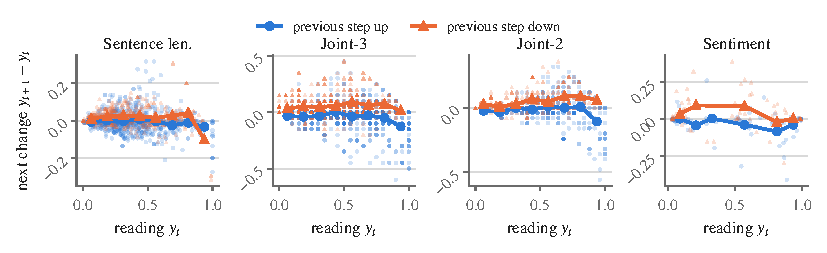
\includegraphics[width=\linewidth]{figs/fig_two_futures.pdf}
\caption{One reading is consistent with two opposite next steps. For each task, the next change against the current reading, split by the direction of the step before it. Faint marks are transitions; the line is the mean of each group in eight equal-width bins. Transitions whose previous step was flat carry no direction and are dropped.}
\label{fig:two_futures}
\end{figure}

\textbf{Findings, why a window helps.} Figure~\ref{fig:two_futures} splits each reading by the direction of the step before it.
At a fixed reading the next change differs with that direction on all four tasks, by +0.100 on Joint-3, +0.070 on Joint-2, +0.058 on sentiment and +0.025 on sentence length.  % m1; figs/_fig_report.json fig_two_futures separation_down_minus_up
The share of transitions dropped for a flat previous step runs from 7\% on sentiment to 66\% on Joint-2, so the display covers a minority of Joint-2 and Joint-3 transitions.  % figs/_fig_report.json n_flat_dropped over n_up+n_down+n_flat_dropped
The separation does not rank the tasks the way the memory gain does: sentence length carries the largest gain in Table~\ref{tab:prediction} and the smallest separation here.  % n_main_013 (+0.603) vs the +0.025 above
Read with \S\ref{sec:exp_memory}, that ordering points at the per-item level rather than the turn-to-turn trend as the larger part of what the window buys.  % m6

\begin{figure}[t]
\centering
\includegraphics[width=\linewidth]{figs/fig_command_channel.pdf}
\caption{The command channel does not move with the state. Applied command against tracking error, coloured by the target. Each target level forms one flat band: the error varies along a band while the command holds its level.}
\label{fig:command_channel}
\end{figure}

\textbf{Findings, what the command channel carries.} On both tasks the applied command takes the value of the target on every recorded transition, 2268 of 2268 on sentence length and 240 of 240 on sentiment.  % m5; figs/_fig_report.json fig_command_channel n_command_equals_target
The tracking error spans $[-0.40, +0.88]$ on sentence length across those same transitions, so the command holds its level over the full range of the error.  % figs/_fig_report.json fig_command_channel
This is the scope statement of \S\ref{sec:exp_analysis} shown on the collection log rather than inferred from a rank test.  % nc_1; nc_8
The two joint tasks record no per-turn scalar command, and their channel was checked by the rank test that subsection cites.  % m5 notes

\begin{figure}[t]
\centering
\includegraphics[width=0.84\linewidth]{figs/fig_lifting_contrast.pdf}
\caption{What a learned lifting costs, by how much structure the readout has. Paired contrast of the linear case over the learned lifting, against the dimension of the attribute readout, with the trajectory count beside each task. Filled: the 95\% interval excludes zero. Dagger: a caveated entry.}
\label{fig:lifting_contrast}
\end{figure}

\textbf{Findings, what a lifting has to find.} The cost of a learned lifting concentrates on the one-dimensional readouts, at +0.599 on CEFR, +0.101 on sentiment and +0.048 on constraint.  % c2; n_main_183 n_main_111 n_main_135
The two multi-dimensional readouts carry +0.014 on Joint-2 and +0.005 on Joint-3, the two smallest entries in the figure.  % n_main_031 n_main_047
The cost does not fall with the number of trajectories: the largest sits on the task fit on 100 trajectories and the smallest on the task fit on 90.  % n_main_183 (n=100) vs n_main_047 (n=90)
The driver is that a one-dimensional readout leaves a lifting little structure to expose, which is the part of the mechanism these seven columns support.  % m4

Together, \uline{the window separates two opposite next steps at one reading, and the cost of a lifting tracks the dimension of the readout rather than the amount of data. The command channel holds its level over the full range of the tracking error, which is why this design cannot measure an action effect.}
